\documentclass[11pt,a4paper]{article}

% Packages
\usepackage[utf8]{inputenc}
\usepackage[T1]{fontenc}
\usepackage{lmodern}
\usepackage{microtype}
\usepackage{amsmath,amssymb}
\usepackage{booktabs}
\usepackage{array}
\usepackage{tabularx}
\usepackage{hyperref}
\usepackage{geometry}
\usepackage{xcolor}
\usepackage{mdframed}
\usepackage{authblk}
\usepackage{parskip}
\usepackage{natbib}
\usepackage{graphicx}
\usepackage{caption}
\captionsetup{font=small, justification=centering}
\usepackage{fontawesome5}
\usepackage{tikz}
\usetikzlibrary{arrows.meta, positioning, fit, backgrounds, calc, shapes.geometric}
\usepackage{todonotes}

\geometry{
  a4paper,
  top=2.5cm,
  bottom=2.5cm,
  left=2.5cm,
  right=2.5cm
}

\hypersetup{
  colorlinks=true,
  linkcolor=blue!60!black,
  citecolor=blue!60!black,
  urlcolor=blue!60!black,
  pdftitle={Distribird: Literature-Informed Prior Distribution Design for Bayesian Model Calibration},
  pdfauthor={P. P. Süli, Gy. Eigner, R. Hollós}
}

% Box style for callouts
\mdfdefinestyle{calloutbox}{
  backgroundcolor=gray!10,
  linecolor=gray!50,
  linewidth=0.8pt,
  innertopmargin=8pt,
  innerbottommargin=8pt,
  innerleftmargin=10pt,
  innerrightmargin=10pt,
  skipabove=\baselineskip,
  skipbelow=\baselineskip
}

% -----------------------------------------------------------------------
\begin{document}

% Title block
\begin{center}
  
\includegraphics[width=0.18\textwidth]{assets/logo.png}\\[6pt]
  {\LARGE\bfseries Distribird}\\[6pt]
  {\large Literature-Informed Prior Distribution Design for Bayesian Model Calibration}\\[10pt]
  Patrik P.\ Süli$^{4,5}$, György Eigner$^{4,5,6}$, Roland Hollós$^{1,2,3}$\\[6pt]
  {\small
  $^1$ HUN-REN AI, Hungary\\ 
  $^2$ HUN-REN Centre for Agricultural Research, Brunszvik u. 2., Martonv\'as\'ar 2462, Hungary\\
  $^3$ Czech Academy of Sciences, Global Change Institute, Czech Republic\\
  $^4$ Doctoral School of Applied Informatics and Applied Mathematics, \\Obuda University, Budapest, Hungary\\
  $^5$ Biomatics and Applied Artificial Intelligence Institute, John von Neumann Faculty of Informatics, Obuda University, Budapest, Hungary\\
  $^6$ Physiological Controls Research Center, Obuda University, Budapest, Hungary\\[4pt]
  suli.patrik@uni-obuda.hu, eigner.gyorgy@uni-obuda.hu, hollos.roland@hun-ren.hu
  }\\[4pt]
  2026\\[4pt]

  \textit{Preprint --- submitted to arXiv}
\end{center}

\begin{center}
\small \faGlobe\, \href{https://distribird.streamlit.app}{\texttt{distribird.streamlit.app}} \quad | \quad \faGithub\, \href{https://github.com/HUN-REN-AI1Science/Distribird}{\texttt{github.com/HUN-REN-AI1Science/Distribird}}
\end{center}

\vspace{0.25em}

% -----------------------------------------------------------------------
\begin{mdframed}[style=calloutbox]
  \textbf{Abstract}\\[4pt]
  Bayesian calibration of process-based models requires the specification of prior distributions
  over model parameters. Despite decades of methodological development, researchers overwhelmingly
  default to uniform priors. The main reason is that constructing
  informative priors from scientific literature is time-consuming and requires both domain and
  statistical expertise. We present \textbf{Distribird}, an agentic web application that automates
  this process. Given a parameter name, physical description, and domain context, Distribird deploys
  a multi-agent LangGraph pipeline that searches Semantic Scholar and OpenAlex in parallel,
  extracts reported numerical values, and fits the best-matching probability distribution via AIC
  model selection from predefined set of distributions. When literature is absent, the system falls back to principled uninformative
  alternatives (Uniform prior or wide Normal), and explicitly communicates the evidential basis
  and confidence level of every prior it produces. Distribird is domain-agnostic and is designed for
 % I removed Jeffreys prior, it sounds right, but it is not part of the application, though it would be quite hard to implement in this framework
  the class of problems where it has the most to offer: physically interpretable parameters in
  process-based models, where domain knowledge exists in published literature and where Bayesian
  calibration with informative priors has clear advantages over uniform-prior alternatives. We
  evaluate the tool on 20~parameters across ten scientific domains, from climate science and
  astrophysics to pharmacokinetics and ecology. Distribird-constructed priors improved MCMC
  sampling efficiency in 80\% of cases (mean ESS ratio 2.78), with gains of up to $13\times$
  in difficult estimation problems and a worst-case penalty of 11\%. Losses occurred exclusively
  on instance-specific parameters whose literature values are not transferable across studies,
  suggesting a clear boundary condition for automated prior construction.
\end{mdframed}

\listoftodos

\todo[inline]{HUN-REN AI, Hungary affiliáció?}

\todo[inline]{The text is great. We need to rewrite some of the sentences, because they sound too much AI. I started the procedure. The em-dashes are quite revealing, and some of the sentence structures are quite revealing as well.}
\todo[inline]{Task: read a similar paper for better structure }

\todo[inline]{Model ellenőrzést beletenni, hogy a kiválasztott priókkal hogyan működik. Maximum posterior kell biztosan, (MAP) -> bele kell tenni, csak az összehasonlítás}

% BullshitBench (out-of-scope detection): see Section~\ref{sec:bullshitbench-design}
% (validity-classification node) and Section~\ref{sec:bullshitbench-eval} (real-LLM
% evaluation across nonsense, theoretical-only, and real parameters).

\vspace{1em}

% -----------------------------------------------------------------------
\section{Introduction}

\subsection{The calibration problem}

Process-based models describe complex natural systems (crop growth, water movement through
soil, biogeochemical cycles, disease spread) using mechanistic equations with parameters that
represent physical or biological quantities. Because many of these parameters cannot be measured
directly, they must be inferred from observations by adjusting parameter values until the model
output matches available data. This process is called model calibration, or inverse modeling \citep{Hollos2022}.

Bayesian calibration is arguably the most principled approach to this
problem, both statistically and philosophically \citep{Gelman2013}. It combines prior knowledge about the parameters with the information
contained in the observed data, and returns a posterior distribution that quantifies not only the
most likely parameter values but also the uncertainty around them. This uncertainty quantification
is critical for decision-making and for honest reporting of model predictions.

\subsection{The prior problem}

The Bayesian approach requires the researcher to specify a prior distribution for each parameter
before seeing the data. This raises an immediate practical question: what prior should be used?

The mathematically convenient answer is to use a uniform prior --- to claim that all parameter
values in a range are equally plausible. This choice is almost universally adopted in practice
\citep{Wallach2021}. It is also almost universally inadequate. \citet{Pericchi1991} demonstrated
that a universally applicable uninformative prior does not exist: uniform priors are not invariant
under reparameterisation, meaning the implied prior changes depending on how the parameter is
expressed. \citet{Gelman1996} showed that the posterior mode under a uniform prior coincides with
the maximum likelihood estimate --- reducing Bayesian inference to the very framework it is
supposed to improve upon. The information loss from ignoring genuine prior knowledge has real
consequences: slower convergence of the sampler, unnecessarily wide credible intervals, and in
data-scarce situations, poorly constrained posteriors that an informative prior would have
regularised.

Informative priors --- priors that encode genuine knowledge about the parameter --- improve all of
these properties. The knowledge needed to construct them exists. It is in the scientific
literature: in papers reporting measured values, in review articles synthesising ranges across
studies, in textbooks describing physical constraints. The problem is not that the knowledge is
absent. The problem is that retrieving and synthesising it is expensive. For a model with twenty
parameters, constructing informative priors from literature may require days of reading.
Researchers default to uniform priors not because they believe them appropriate, but because the
alternative is too costly.

This gap between knowing the problem and having a scalable solution has persisted for more than
thirty years.

\subsection{Large language models as a solution pathway}

Recent advances in large language models (LLMs) with agentic search capability have created a new
option. An LLM agent can search scientific databases, retrieve relevant papers, extract reported
numerical values, and synthesise them into a probability distribution --- automatically, and at a
cost that makes the process practical for routine use.

We present Distribird, a web application and Python library that implements this pipeline. Distribird is
not a general-purpose prior elicitation tool. It is designed specifically for the class of
problems where literature-based prior construction is most appropriate and most impactful:
process-based models with physically interpretable parameters, active publishing communities, and
genuine prior knowledge encoded in the scientific record.

% -----------------------------------------------------------------------
\section{Conditions of Applicability}

Distribird produces its best results under the following conditions, which define the class of
problems the tool is designed for:

\begin{itemize}
  \item \textbf{Physically interpretable parameters:} The parameter has a physical or biological
    interpretation that is discussed in the scientific literature --- for example, a maximum
    photosynthesis rate, a root depth, a transmission coefficient, or a thermal threshold.

  \item \textbf{Literature-active domain:} The domain has an active publishing community, so that
    relevant papers can be found by automated search.

  \item \textbf{Univariate distributions:} The parameter can be described by a standard univariate
    probability distribution (Normal, truncated Normal, Beta, Gamma, Log-Normal). Parameters with
    complex multimodal behaviour are outside the current scope.

  \item \textbf{Known physical bounds:} Physical bounds on the parameter are known or can be
    reasoned about by the user, so that the fitted distribution can be constrained appropriately.
\end{itemize}

When these conditions are not fully met, Distribird degrades gracefully: it communicates the
evidential basis of its output explicitly, flags low-confidence results, and falls back to
principled uninformative alternatives rather than producing false confidence. The confidence
hierarchy is described in Section~\ref{sec:confidence}.

\begin{mdframed}[style=calloutbox]
  \textbf{What Distribird is not designed for}\\[4pt]
  Distribird is not designed for parameters without physical interpretation (e.g.\ neural network
  weights), purely empirical tuning coefficients with no literature base, or parameters whose
  behaviour is fundamentally multivariate. For these cases, other approaches --- prior predictive
  checks, expert elicitation, or sensitivity analysis --- remain more appropriate. To prevent
  silent misuse, the pipeline classifies each request and explicitly flags out-of-scope inputs
  (Section~\ref{sec:bullshitbench-design}); we evaluate this defence in
  Section~\ref{sec:bullshitbench-eval}.
\end{mdframed}

% -----------------------------------------------------------------------
\section{System Design}

\subsection{Overview}

Distribird is implemented as a Python~3.10+ package distributed via \href{https://pypi.org/project/distribird/}{PyPI} and exposing two user-facing interfaces: a REST~API built on FastAPI and an interactive Streamlit web application. Both interfaces delegate to the same core pipeline, ensuring identical behaviour regardless of access method. The system is configured through environment variables, making deployment straightforward via Docker or direct installation.

The user provides a \texttt{ParameterInput} object specifying the parameter name, a plain-language physical description, the measurement unit, a domain context string (e.g.\ ``Biome-BGCMuSo maize crop modelling, Central European conditions''), and optional physical constraints (lower bound, upper bound). For example:

\begin{verbatim}
  ParameterInput(
      name="TMAX",
      description="Maximum temperature for photosynthesis",
      unit="°C",
      domain_context="Biome-BGCMuSo maize, Central Europe",
      constraints=ConstraintSpec(lower_bound=30.0, upper_bound=50.0)
  )
\end{verbatim}

\noindent The system returns a \texttt{PipelineResult} containing the fitted prior distribution, its confidence level, the number of contributing sources, all search queries attempted, the full list of retrieved papers with extracted values, an optional enrichment context, and --- when multi-agent deliberation is enabled --- the moderator's rationale and any excluded papers. A simplified example:

\begin{verbatim}
  PipelineResult(
      prior=FittedPrior(
          family="truncated_normal",
          params={"mu": 40.5, "sigma": 3.2, "a": 30.0, "b": 50.0},
          confidence="high",
          is_informative=True,
          n_sources=6
      ),
      papers_found=16,
      values_extracted=8,
      search_queries=["maize maximum photosynthesis temperature", ...]
  )
\end{verbatim}

\noindent This complete provenance chain allows the user to audit every step from literature search to final distribution.

\subsection{Multi-agent LangGraph pipeline}

The core of Distribird is a LangGraph \texttt{StateGraph} that orchestrates a multi-agent pipeline with two feedback loops and a conditional forward path. Unlike a directed acyclic graph, the pipeline permits cycles: when initial evidence is insufficient, the graph routes back to earlier nodes for refinement before proceeding to synthesis. All nodes read from and write to a shared \texttt{PipelineState} typed dictionary that follows the blackboard pattern --- an append-only message log (\texttt{BlackboardMessage}) through which nodes communicate discoveries, terminology updates, query suggestions, cross-references, and warnings without direct coupling.

\subsubsection{Pipeline overview}

Figure~\ref{fig:pipeline} illustrates the complete graph topology, including two feedback loops, one conditional forward path, and the multi-agent search subsystem. The pipeline comprises ten primary processing nodes (including a terminal validity-classification node, Section~\ref{sec:bullshitbench-design}) and three refinement nodes, connected by two routing functions that implement the conditional logic.

\begin{figure}[!htbp]
\centering
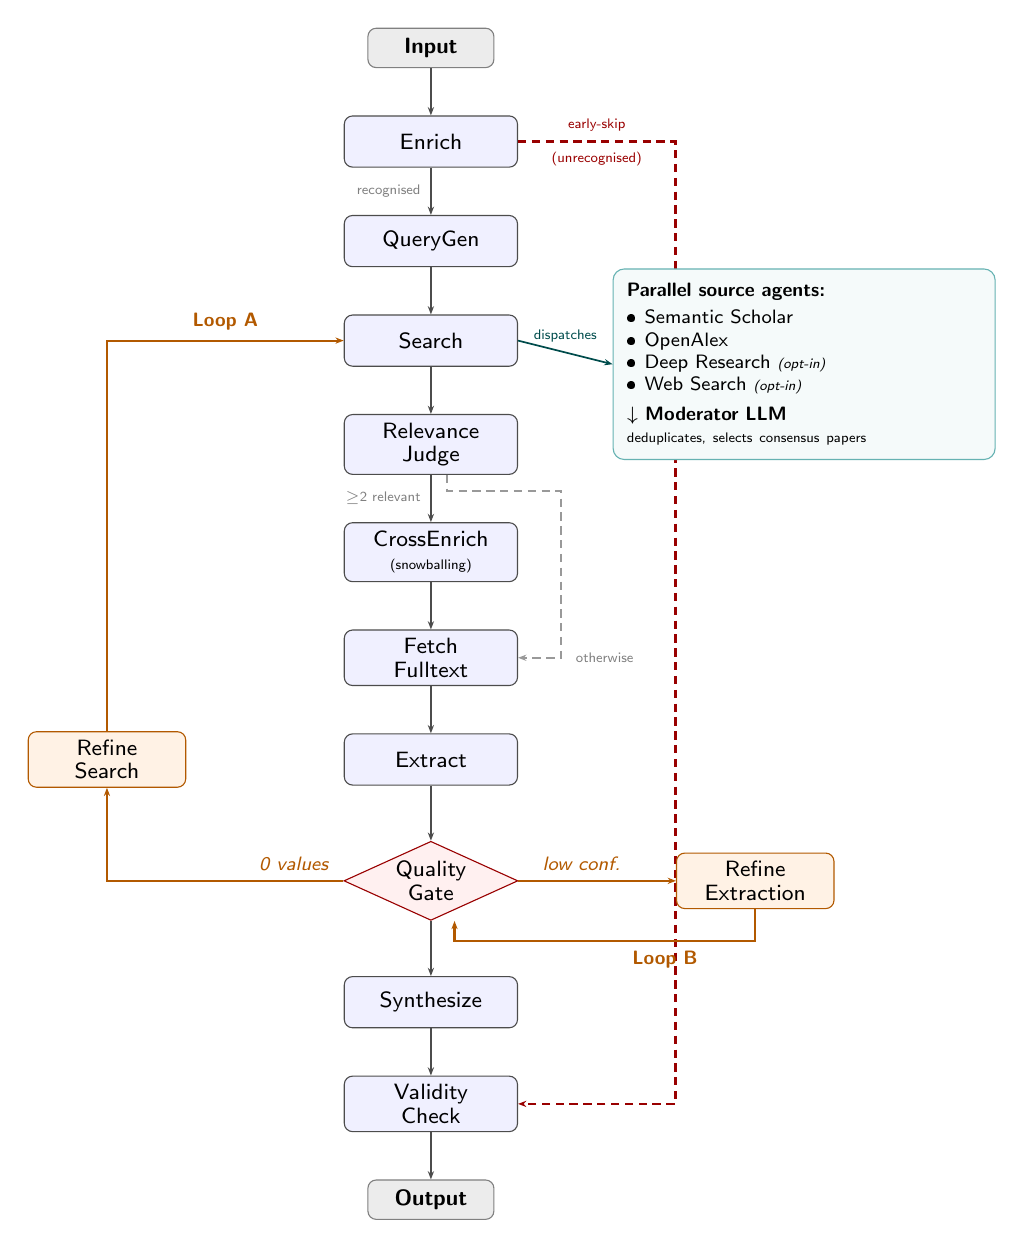
\begin{tikzpicture}[
  node distance=0.6cm,
  >={Stealth[length=3pt]},
  mainnode/.style={
    rectangle, rounded corners=3pt, draw=black!70, fill=blue!6,
    minimum width=2.2cm, minimum height=0.65cm,
    font=\footnotesize\sffamily, align=center, inner sep=3pt
  },
  refinenode/.style={
    rectangle, rounded corners=3pt, draw=orange!70!black, fill=orange!10,
    minimum width=2.0cm, minimum height=0.65cm,
    font=\footnotesize\sffamily, align=center, inner sep=3pt
  },
  gatenode/.style={
    diamond, draw=red!60!black, fill=red!6,
    minimum width=1.0cm, minimum height=0.6cm,
    font=\footnotesize\sffamily, align=center, inner sep=1pt,
    aspect=2.2
  },
  termnode/.style={
    rectangle, rounded corners=3pt, draw=black!50, fill=gray!15,
    minimum width=1.6cm, minimum height=0.5cm,
    font=\footnotesize\sffamily\bfseries, align=center, inner sep=3pt
  },
  looplabel/.style={font=\scriptsize\sffamily\itshape, text=orange!70!black},
  mainedge/.style={draw, ->, thick, black!70},
  loopedge/.style={draw, ->, thick, orange!70!black},
  condlabel/.style={font=\tiny\sffamily, text=black!50},
]

% ============================================================
% MAIN VERTICAL FLOW
% ============================================================
\node[termnode] (start) {Input};
\node[mainnode, below=of start] (enrich) {Enrich};
\node[mainnode, below=of enrich] (querygen) {QueryGen};
\node[mainnode, below=of querygen] (search) {Search};
\node[mainnode, below=of search] (relevance) {Relevance\\[-1pt]Judge};
\node[mainnode, below=of relevance] (crossenrich) {CrossEnrich\\[-1pt]{\tiny(snowballing)}};
\node[mainnode, below=of crossenrich] (fulltext) {Fetch\\[-1pt]Fulltext};
\node[mainnode, below=of fulltext] (extract) {Extract};
\node[gatenode, below=0.7cm of extract] (qgate) {Quality\\[-1pt]Gate};
\node[mainnode, below=0.7cm of qgate] (synthesize) {Synthesize};
\node[mainnode, below=of synthesize] (validity) {Validity\\[-1pt]Check};
\node[termnode, below=of validity] (output) {Output};

% ============================================================
% MAIN FLOW EDGES
% ============================================================
\draw[mainedge] (start) -- (enrich);

% --- Conditional: Enrich → QueryGen OR ValidityCheck (early-skip) ---
% Code: route_after_enrich() — if LLM does not recognize parameter, skip directly
% to validity_check to avoid wasting search/extract/synthesize compute.
\draw[mainedge] (enrich) -- node[condlabel, left] {recognised} (querygen);
\draw[mainedge, densely dashed, red!60!black]
  (enrich.east) -- ++(2.0,0)
  node[condlabel, above, midway, text=red!60!black] {early-skip}
  node[condlabel, below, midway, text=red!60!black] {(unrecognised)}
  |- (validity.east);

\draw[mainedge] (querygen) -- (search);
\draw[mainedge] (search) -- (relevance);

% --- Conditional: RelevanceJudge → CrossEnrich OR FetchFulltext ---
% Code: route_after_deliberation() — if ≥2 high-relevance papers → cross_enrich, else → fetch_fulltext
\draw[mainedge] (relevance) -- node[condlabel, left] {$\geq$2 relevant} (crossenrich);
\draw[mainedge, densely dashed, black!40]
  ([xshift=0.2cm]relevance.south) -- ++(0,-0.2)
  -| ([xshift=0.55cm]fulltext.east) -- (fulltext.east);
\node[condlabel] at ([xshift=1.1cm]fulltext.east) {otherwise};

\draw[mainedge] (crossenrich) -- (fulltext);
\draw[mainedge] (fulltext) -- (extract);
\draw[mainedge] (extract) -- (qgate);

% --- Conditional: QualityGate → Synthesize OR RefineSearch OR RefineExtraction ---
\draw[mainedge] (qgate) -- (synthesize);
\draw[mainedge] (synthesize) -- (validity);
\draw[mainedge] (validity) -- (output);

% ============================================================
% MULTI-AGENT SEARCH (annotation to the right of Search node)
% Shows what happens INSIDE search_node
% ============================================================
% Simple callout box listing the agents and moderator
\node[draw=teal!60, rounded corners=4pt, fill=teal!4,
      text width=4.5cm, font=\scriptsize\sffamily,
      inner sep=5pt, align=left,
      right=1.2cm of search, yshift=-0.3cm]
  (agentbox) {%
    \textbf{Parallel source agents:}\\[2pt]
    \textbullet~Semantic Scholar\\
    \textbullet~OpenAlex\\
    \textbullet~Deep Research {\tiny\itshape(opt-in)}\\
    \textbullet~Web Search {\tiny\itshape(opt-in)}\\[3pt]
    \textbf{$\downarrow$ Moderator LLM}\\
    {\tiny deduplicates, selects consensus papers}
  };
\draw[draw, ->, semithick, teal!60!black]
  (search.east) -- (agentbox.west)
  node[condlabel, above, midway, text=teal!60!black] {dispatches};

% ============================================================
% LOOP A: QualityGate → RefineSearch → Search
% Code: quality_gate --[0 values]--> refine_search --> search
% ============================================================
\node[refinenode, left=2.0cm of extract] (refinesearch) {Refine\\[-1pt]Search};

\draw[loopedge]
  (qgate.west) -| node[looplabel, above right, pos=0.2] {0 values} (refinesearch.south);
\draw[loopedge]
  (refinesearch.north) |- node[looplabel, above, pos=0.75] {\textbf{Loop A}} (search.west);

% ============================================================
% LOOP B: QualityGate → RefineExtraction → QualityGate
% Code: quality_gate --[low conf.]--> refine_extraction --> quality_gate
% ============================================================
\node[refinenode, right=2.0cm of qgate] (refineextract) {Refine\\[-1pt]Extraction};

\draw[loopedge]
  (qgate.east) -- node[looplabel, above, pos=0.4] {low conf.} (refineextract.west);
\draw[loopedge]
  (refineextract.south) -- ++(0,-0.4) -|
  node[looplabel, below, pos=0.15] {\textbf{Loop B}} ([xshift=0.3cm]qgate.south);

\end{tikzpicture}
\caption{Distribird LangGraph pipeline. Two feedback loops (A, B), one conditional forward path
(cross-enrichment), and one early-skip path (red dashed) from Enrich directly to Validity~Check.
When the enrichment LLM clearly does not recognise the requested parameter, the pipeline bypasses
all subsequent search, extraction, and synthesis work and proceeds straight to classification ---
saving roughly 90\% of the wall-clock cost on out-of-scope requests. The Search node internally
dispatches to parallel source agents whose outputs are reconciled by a Moderator LLM. The terminal
Validity~Check node classifies the request as VALID, SUSPICIOUS, LIKELY\_INVALID, or UNKNOWN
(Section~\ref{sec:bullshitbench-design}).}
\label{fig:pipeline}
\end{figure}

\subsubsection{Pipeline nodes and feedback loops}
\label{sec:feedback}

The pipeline comprises ten primary processing nodes --- Enrich (parameter semantics expansion), QueryGen (search query generation), Search (parallel API queries), RelevanceJudge (paper scoring), CrossEnrich (citation snowballing), FetchFulltext (PDF retrieval and parsing), Extract (numerical value extraction), QualityGate (routing logic), Synthesize (distribution fitting), and ValidityCheck (out-of-scope classification, Section~\ref{sec:bullshitbench-design}) --- connected by two feedback loops and one conditional forward path that allow the pipeline to iteratively improve its results when initial evidence is insufficient:

\begin{itemize}
  \item \textbf{Loop~A --- Search refinement.} When the quality gate finds zero extracted values but papers were retrieved (indicating that the search found relevant literature but extraction failed to locate numerical data), the pipeline routes to a \texttt{RefineSearch} node. This node analyses the summaries of retrieved papers and generates refined search queries targeting more specific experimental or calibration studies. Control then returns to the Search node. This loop may execute up to two iterations (configurable via \texttt{search\_refinement\_max}).

  \item \textbf{Conditional path --- Cross-enrichment.} After relevance judgment, if the iteration budget permits and at least two high-relevance papers have been identified, the pipeline routes through CrossEnrich (citation snowballing) before fetching full texts; otherwise, it skips directly to FetchFulltext. This is a conditional forward path, not a feedback loop --- it does not cycle back to an earlier node. The cross-enrichment step is executed at most once per pipeline invocation (\texttt{cross\_enrichment\_max\,=\,1}).

  \item \textbf{Loop~B --- Extraction refinement.} When the quality gate finds extracted values but none are high-confidence and the coefficient of variation exceeds~1.5 (indicating high disagreement among sources), the pipeline routes to a \texttt{RefineExtraction} node that uses web-assisted search to locate additional confirming or disconfirming evidence. Control returns to the quality gate for re-evaluation. This loop may execute once (\texttt{extraction\_refinement\_max\,=\,1}).
\end{itemize}

\noindent An \texttt{IterationBudget} object tracks the number of iterations consumed by each loop and enforces a global cap on total LLM calls (default: 30), guaranteeing termination even when both loops and the conditional path are activated in the same invocation. The budget is checked at every conditional routing point; when exhausted, the pipeline proceeds directly to synthesis with whatever evidence has been accumulated.


\subsection{Validity classification: detecting out-of-scope requests}
\label{sec:bullshitbench-design}

A literature-grounded prior is only meaningful for parameters whose values are reported in the scientific record. Two failure modes lie outside Distribird's contract: fabricated or non-scientific names (e.g.\ a typo, a pseudoscientific term, or a placeholder), and parameters that genuinely belong to a model but are not empirically measured (calibration weights, latent state covariances, software-version-specific tuning factors). In both cases the synthesizer's tiered fallback already produces a wide uninformative prior with low confidence, but it does so silently, which risks downstream users mistaking the placeholder for evidence-backed guidance. The pipeline closes this gap by classifying every request into one of four categories --- \textsc{Valid}, \textsc{Suspicious}, \textsc{Likely\_Invalid}, or \textsc{Unknown} --- using a two-stage gating strategy: an \emph{early-skip} immediately after enrichment that prevents wasted compute on clearly invalid requests, and a \emph{terminal classifier} that issues the final verdict using all collected signals. The combined design adds at most one extra LLM call beyond the standard pipeline.

The early-skip route examines the enrichment LLM's self-reports as soon as they become available. The \texttt{PARAMETER\_ENRICHMENT} prompt is extended with three additional fields --- whether the LLM recognises the parameter as an established scientific quantity, the LLM's confidence in that recognition, and whether the parameter is empirically measurable rather than theoretical. When the LLM responds with \texttt{is\_recognized\_parameter=False} at \texttt{none} or \texttt{low} confidence, the routing function \texttt{route\_after\_enrich} forwards the state directly to the terminal validity-check node, bypassing query generation, the multi-agent search, full-text retrieval, extraction, the quality gate, and synthesis. Because the search and extraction stages dominate the wall-clock cost of a parameter request (typically 80--95\% of the total runtime in our benchmarks), this short-circuit prevents the system from running expensive paper retrieval and LLM-driven extraction for inputs that the model itself has already classified as nonsense. Requests that pass the early gate proceed through the standard pipeline and are subjected to the terminal classifier with the full evidence base in hand.

The terminal classifier consumes signals collected throughout the run: the enrichment self-reports, the number of refined queries tried, the number of papers retrieved, the number of values extracted, and the confidence of the fitted prior. A small set of pure-Python heuristic rules combines these signals into a passive verdict. A request that reaches the classifier through the early-skip path is marked \textsc{Likely\_Invalid} (no literature, no terminology, unrecognised name). A request whose enrichment reports the parameter as not empirically measured (or whose empirical status is uncertain) where literature was found but no values could be extracted is marked \textsc{Suspicious}: the parameter exists in some published model but cannot be grounded in measurement. A request with a high- or medium-confidence informative prior, recognised terminology, and at least two extracted values is marked \textsc{Valid}; the gate requires the recognition signal to be strictly true (rather than merely not false), so an LLM that is uncertain about the parameter's identity still falls through to the probe.

When the passive verdict is \textsc{Suspicious}, the node calls a dedicated \texttt{PARAMETER\_VALIDITY\_PROBE} LLM that receives the enrichment self-flags, the pipeline observations, and a description of the four verdicts. The probe can refine the verdict in either direction --- upgrading clear nonsense to \textsc{Likely\_Invalid} or confirming theoretical-only parameters as \textsc{Suspicious} --- but cannot override a \textsc{Valid} or \textsc{Likely\_Invalid} verdict already reached by the passive heuristics. The probe is gated by both the iteration budget and an \texttt{enable\_validity\_probe} setting, so users who require fully offline operation can disable it. The verdict, the passive signals that produced it, and the probe's reason are exposed on the \texttt{PipelineResult} via the \texttt{parameter\_validity}, \texttt{validity\_reason}, \texttt{validity\_signals}, and \texttt{is\_empirical} fields, and a human-readable warning of the form ``Parameter validity: \textsc{suspicious} --- \textit{reason}'' is appended to \texttt{PipelineResult.warnings} so that command-line and Streamlit consumers see the verdict at a glance.

\subsection{Literature search}

The search subsystem queries two academic APIs in parallel. \textit{Semantic Scholar} provides citation-graph metadata, abstracts, and open-access PDF links via its Graph~API; \textit{OpenAlex} provides an independent index with complementary coverage, reconstructing abstracts from its inverted-index representation. Both APIs are filtered to open-access papers only, ensuring that full-text retrieval is feasible.

Two additional source agents are available as optional complements. A \textit{deep-research agent} delegates to an LLM with web-search capabilities (configurable model, default OpenAI's \texttt{o4-mini-deep-research}) to discover papers that may not be indexed by the academic APIs; its results are verified against Semantic Scholar before inclusion to prevent hallucinated references. A \textit{web search agent} performs a similar verification-backed LLM search using a general-purpose web-search prompt. Both agents contribute \texttt{AgentFinding} objects to the deliberation process alongside the API-based agents.

\subsection{Prior fitting and confidence hierarchy}
\label{sec:confidence}

The distribution fitting strategy is tiered according to the amount of evidence recovered, ensuring that the statistical method matches the information content of the data:

\begin{table}[!htbp]
\centering
\caption{Tiered prior fitting strategy based on available evidence.}
\label{tab:confidence}
\small
\begin{tabularx}{\linewidth}{@{}l>{\raggedright\arraybackslash}Xll@{}}
  \toprule
  \textbf{Evidence} & \textbf{Method} & \textbf{Confidence} & \textbf{Fallback?} \\
  \midrule
  $\geq 5$ values & AIC model selection across five candidate families: Normal, Truncated Normal, Gamma, Log-Normal, and Beta. The family minimising AIC is selected. For distributions requiring positive support (Gamma, Log-Normal), only positive values are considered; Beta fitting requires user-specified bounds. & High & No \\[4pt]
  2--4 values & Moment matching to a Truncated Normal with the standard deviation widened by a factor of~1.5. A minimum-width floor is imposed: $\sigma \geq \max(0.05\,|\mu|,\; 0.05\,(u - l))$, where $u$ and $l$ are the upper and lower bounds, to prevent overconfident priors from sparse data. & Medium & No \\[4pt]
  1 value & Wide Normal centred on the single reported value, with $\sigma$ set to a conservative fraction of the plausible range. & Low & No \\[4pt]
  0 values & Uniform prior over the user-specified bounds, or a wide Truncated Normal centred at the midpoint of the bounds with $\sigma = (u - l)/4$. & None & Yes \\
  \bottomrule
\end{tabularx}
\end{table}

\todo[inline]{We have to be explicit on the distributions for the fitting. Ne táblzatban legyen, hanem felette legyen kifejtve mikor használjuk az AIC-ot, Momentumot, meg mikor Normal, Gamma, Beta, stb...}

\noindent All fitted distributions are constrained to respect user-specified physical bounds. When sample sizes or uncertainties are reported alongside extracted values, inverse-variance weighting is applied during fitting. The confidence level is recorded in the \texttt{FittedPrior} object and propagated through all export formats, ensuring that downstream users can distinguish empirically grounded priors from uninformative fallbacks.

\subsection{Export formats}

Distribird exports priors in three formats designed for direct integration into common Bayesian calibration workflows:

\begin{itemize}
  \item \textbf{JSON} --- a structured record containing the parameter name, distribution family, fitted parameters, confidence level, informative/uninformative flag, fitting rationale, number of contributing sources, and a citation list with title, DOI, year, and authors for each paper. Batch exports include a version tag and run metadata.

  \item \textbf{Python} --- an executable \texttt{scipy.stats} script that defines a sampling function for each parameter, imports \texttt{numpy} and \texttt{scipy}, and generates a configurable number of random draws (default: 10\,000). The generated code is compatible with PyMC, emcee, and custom MCMC samplers.

  \item \textbf{R} --- an executable R script using base distribution functions (\texttt{rnorm}, \texttt{rgamma}, \texttt{rlnorm}, \texttt{rbeta}, \texttt{runif}) and the \texttt{truncnorm} package for truncated normal sampling. The script is ready for use with BayesianTools, FME, or custom samplers.
\end{itemize}

\noindent All three formats embed the complete provenance chain --- from search queries through paper citations to the fitting rationale --- so that the prior's evidential basis is preserved alongside its numerical specification.


% -----------------------------------------------------------------------
\section{Experimental Evaluation}
\label{sec:exp-eval}

We tested whether Distribird's literature-informed priors improve Bayesian parameter estimation compared to the standard practice of using uniform (``I don't know'') priors. The experiment covered 20~parameters across ten scientific domains, using real publicly available datasets.

\subsection{Experimental design}

For each parameter, we ran the same Bayesian model twice: once with the Distribird-constructed prior and once with a uniform prior over the same bounds. Both runs used identical data, the same sampling algorithm \citep[NUTS;][]{Hoffman2014}, and the same configuration (2\,000~samples, 4~parallel chains, fixed random seed).

We measure success using the \emph{ESS ratio}: the effective number of independent samples produced by the informed run divided by the flat run. An ESS ratio above~1 means the informed prior helped the sampler work more efficiently; below~1 means the uniform prior performed better. We call an ESS ratio above~1 an informed ``win.''

Beyond raw efficiency, we also track two reliability indicators: whether the sampler encountered numerical problems (divergent transitions) and whether the chains agreed with each other ($\hat{R}$ convergence statistic \citep{Vehtari2021}). We define a \emph{no-harm} outcome as one where the informed prior did not make either reliability indicator worse, even if it did not improve ESS. This distinction matters in practice: a slightly slower but reliable sampler is far preferable to a faster one that produces untrustworthy results.

\subsection{Use cases and datasets}
\label{sec:usecases}

Ten scientific domains were selected to span a broad range of model types and data characteristics. Within ecology, two independent predator--prey systems were tested, yielding 11~use cases and 20~parameters in total. All datasets are real, publicly available, and require no registration to access.

\begin{table}[!htbp]
\centering
\caption{Experimental use cases and datasets. $n$: number of observations.}
\label{tab:usecases}
\footnotesize
\setlength{\tabcolsep}{4pt}
\begin{tabular}{@{}llllr@{}}
  \toprule
  \textbf{Domain} & \textbf{Parameters} & \textbf{Model / Likelihood} & \textbf{Data source} & $n$ \\
  \midrule
  Climate & $r_{\text{eff}}$, AOD & Linear regr.\ / Normal & AERONET \citep{Holben1998} & 50 \\
  Pharmacokinetics & clearance, $V_d$ & Bateman eq.\ / Normal & Theoph \citep{Boeckmann1994} & 132 \\
  Hydrology & $f_c$, $K_{\text{sat}}$ & Bucket / Normal & NRFA stn.\ 39001 & 366 \\
  Structural Eng. & $E$, $\zeta$ & Eigenfreq.\ / Normal & Yonghe \citep{Li2019} & 216 \\
  Epidemiology & incub., infect.\ period & SEIR / Neg.\ Binom. & OWID \citep{Mathieu2021} & 60 \\
  Astrophysics & $H_0$, $\Omega_m$ & Distance mod.\ / Normal & Pantheon+ \citep{Scolnic2022} & 1701 \\
  Ecology (Isle R.) & moose $r$ & Lotka--Volterra / LogN & \citet{Vucetich2012} & 58 \\
  Ecology (YNP) & elk $r$ & Lotka--Volterra / LogN & \citet{Hobbs2023} & 28 \\
  Geophysics & perm., porosity & Kozeny--Carman / LogN & USGS \citep{Nelson2003} & 26 \\
  Robotics & friction, inertia & Inv.\ dynamics / Normal & KUKA \citep{Meier2016} & 700 \\
  Economics & stickiness, $\phi_\pi$ & NK Phillips--Taylor / Normal & FRED \citep{FRED2026} & 60 \\
  \bottomrule
\end{tabular}
\end{table}

\noindent Each use case employed a domain-appropriate generative model in which the parameters of interest appear as priors. Model structures range from simple linear regression (climate) through ordinary differential equation solvers (ecology) to the flat $\Lambda$CDM distance--redshift relation (astrophysics).

\subsection{Prior construction results}

Distribird was run on all 20~parameters with default settings (context enrichment, Semantic Scholar and OpenAlex search, relevance judgment, and citation snowballing enabled; deep-research and web-search agents disabled). Table~\ref{tab:priors} in Appendix~\ref{app:tables} lists the full set of constructed priors.

Of the 20~parameters, 19 received informative priors (95\%) and one --- the elk intrinsic growth rate (Ecology~(YNP), elk~$r$ in Table~\ref{tab:priors}) --- received an uninformative fallback (wide truncated Normal centred at the midpoint of the bounds). The confidence breakdown was: 15~high confidence ($\geq 5$ extracted values, best distribution selected automatically), 4~medium (2--4~values, moment-matched), and 1~none (zero values, fallback prior). The richest prior evidence base was the COVID-19 incubation period (Epidemiology in Table~\ref{tab:usecases}), where Distribird extracted 105~reported values from 27~papers.

\subsection{MCMC comparison results}
\label{sec:mcmc}

Table~\ref{tab:mcmc} in Appendix~\ref{app:tables} presents the full per-parameter results. Across the 20~parameters, informed priors won on 16 (80\%), with a mean ESS ratio of~2.78 and a median of~1.28. All informed-prior runs converged successfully. The total number of numerical problems (divergent transitions) was substantially lower under informed priors (264 vs.\ 1\,933 across all runs). Figure~\ref{fig:ess_scatter} visualises the comparison.

\begin{figure}[!htbp]
\centering
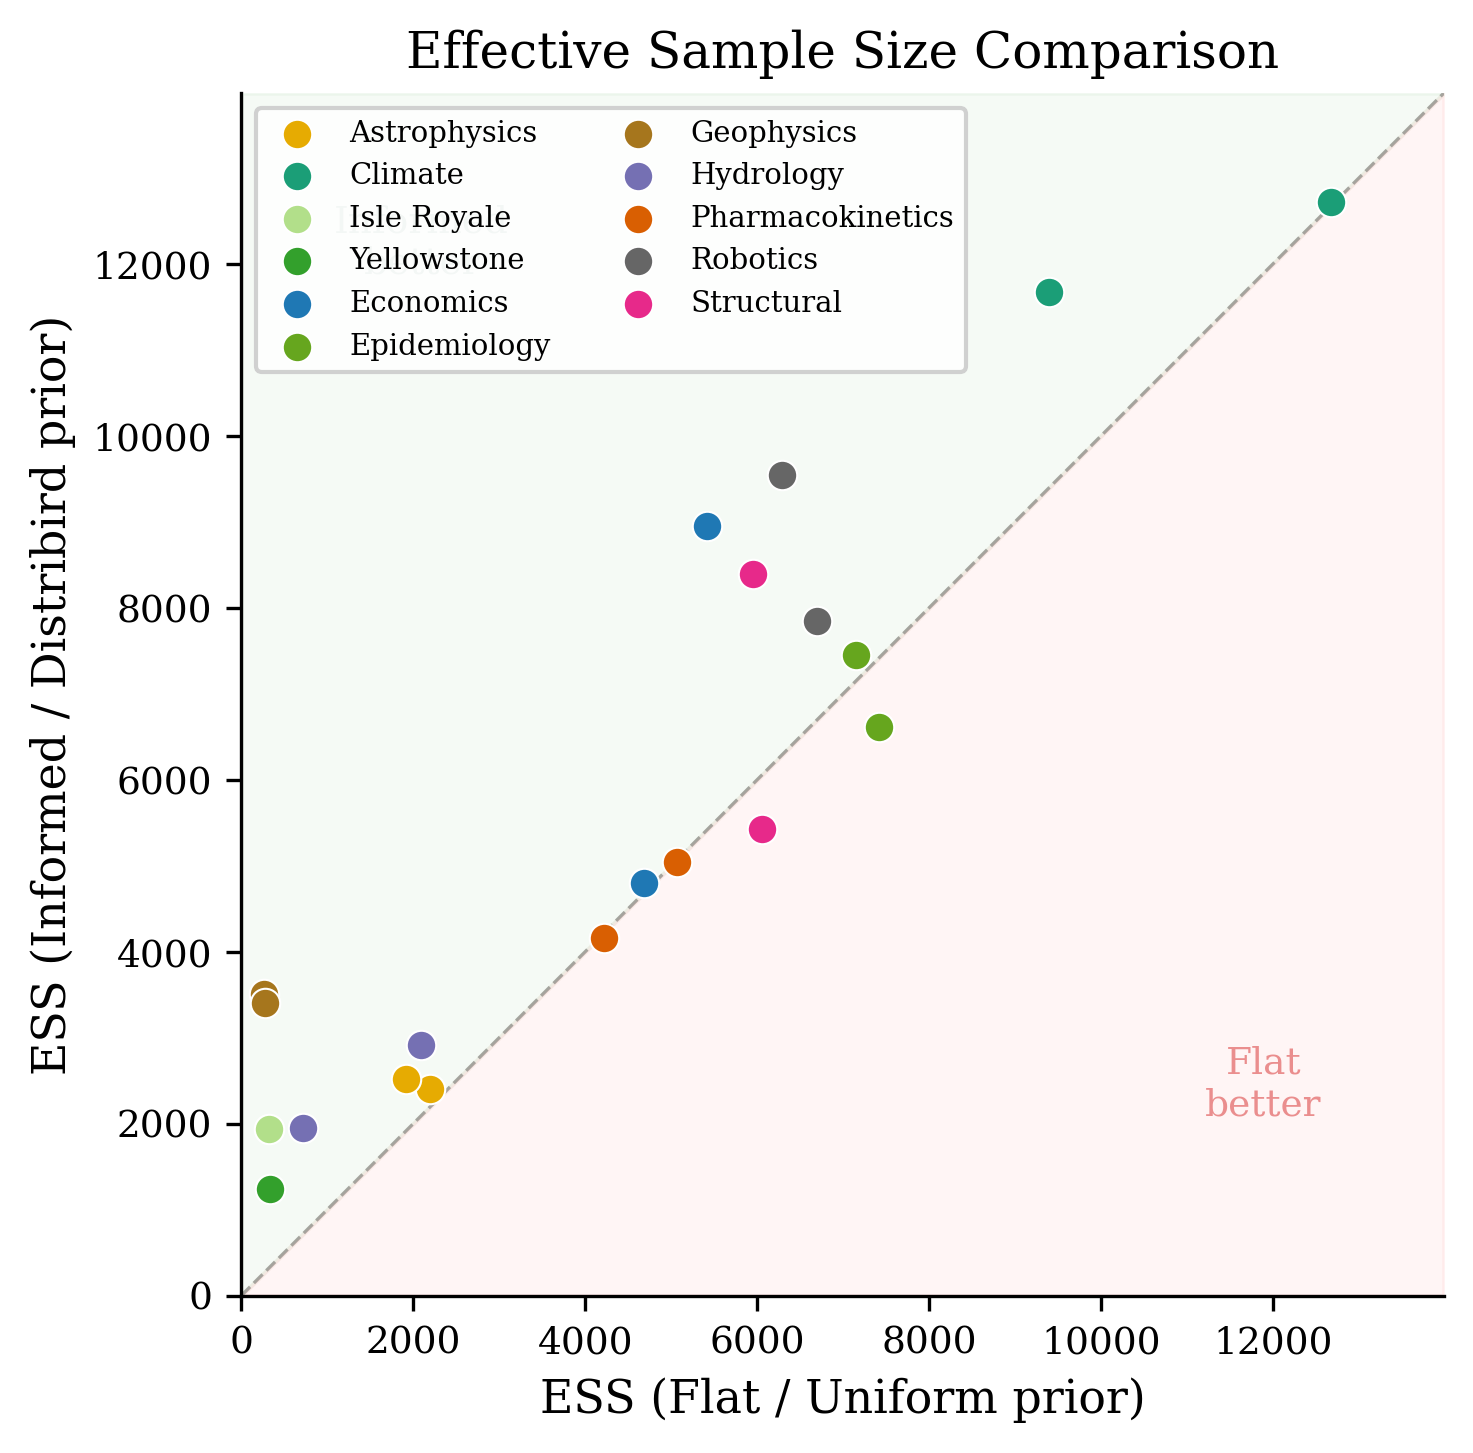
\includegraphics[width=0.7\linewidth]{figures/ess_scatter.png}
\caption{Effective sample size under informed priors (vertical axis) vs.\ flat priors (horizontal axis) for the 20~analysed parameters, coloured by scientific domain. Points above the diagonal indicate that the informed prior improved sampling efficiency.}
\label{fig:ess_scatter}
\end{figure}

The size of the improvement varied with the difficulty of the estimation problem. The largest gains appeared in geophysics (ESS ratios of 13.0 and 12.5), where the parameter space spans four orders of magnitude and the uniform prior spreads probability mass too thinly for the sampler to find the right region quickly. The ecology predator--prey models showed the second-largest gains (ESS ratios of 3.8--6.0), where the complex dynamics make the estimation landscape difficult to navigate without prior guidance.

The improvement is strongly asymmetric: when informed priors help, they help a lot (up to $13\times$ faster sampling); when they do not help, the penalty is negligible. The four losses --- pharmacokinetics clearance (0.99), pharmacokinetics $V_d$ (0.99), structural damping ratio (0.90), and epidemiology incubation period (0.89) --- represent deficits of only 0.5\%--11\%. In every one of these cases, the informed prior either matched or improved the reliability diagnostics (convergence and divergent transitions). The no-harm rate --- the fraction of parameters where the informed prior did not worsen any reliability diagnostic --- was 19/20 (95\%). The single exception (economics inflation response coefficient) showed a negligible $\hat{R}$ increase of 0.001, well within acceptable bounds. In practical terms, using an informed prior never made things worse in a way that mattered.

\subsection{Why the informed prior lost: parameter transferability}

The four losses reveal an important pattern about when literature-based priors work best.

The key distinction is between \emph{transferable} and \emph{instance-specific} parameters. A transferable parameter describes a property of a \emph{class} --- a species, a material, a physical law --- so that a measurement made in one study directly informs the same quantity in another. The Hubble constant is the clearest example: every measurement in the literature constrains the same universal value. Material properties (sandstone porosity), species-level traits (moose growth rate), and atmospheric quantities (aerosol optical depth) are similarly transferable. For these parameters, Distribird achieved its strongest results (ESS ratios of 1.0--13.0), because the literature describes exactly the quantity being calibrated.

Instance-specific parameters, by contrast, depend on the particular system under study, and published values from other systems do not directly transfer:

\begin{itemize}
  \item \textbf{Pharmacokinetics.} Theophylline clearance and volume of distribution depend on the specific patient cohort, dose, and formulation. Literature values aggregate across different clinical conditions --- the resulting prior is correctly placed but encodes between-study variability that does not match the specific Theoph dataset. With 132~dense observations, the data overwhelms any prior regardless.

  \item \textbf{Structural engineering.} The damping ratio $\zeta$ of the Yonghe Bridge depends on that bridge's construction, age, and condition. Published damping ratios from other bridges inform the right order of magnitude, but not the specific value.

  \item \textbf{Epidemiology.} COVID-19 incubation period varies across viral lineages and populations. The 110~values Distribird extracted span multiple SARS-CoV-2 variants, introducing spread that may not represent the specific wave in the calibration data.
\end{itemize}

In all four cases, Distribird correctly found and synthesised the literature --- the priors were well-centred and received high confidence scores. The tool did not fail; the knowledge simply was not transferable. The evidence describes a \emph{population of instances} rather than the specific instance being calibrated. Even so, the resulting ESS penalty was small (0.5\%--11\%), and reliability diagnostics were never worsened.

This pattern suggests a practical rule of thumb: Distribird is most effective when the parameter represents a property of a class rather than a property of a specific instance. Among the 16~transferable parameters in this experiment, the informed-prior win rate was 100\%.

\subsection{Extraction validation}

To assess the quality of the LLM extraction step independently of MCMC performance, we audited the 473~numerical values extracted across all 20~parameters. Of the 138~contributing source papers, 133 (96.4\%) had valid DOIs that resolve to the claimed publication. All 473~extracted values included a natural-language context string describing where in the paper the value was found (e.g.\ ``Alpha variant; pooled mean incubation period, 95\%~CI 4.53--5.30''). Of the 473~values, 424 (89.6\%) fell within the user-specified physical bounds for their parameter. The 49~out-of-bounds values occurred primarily in parameters with narrow bounds and broad literature coverage (e.g.\ lognormal-distributed quantities where some reported values exceed the upper constraint); these values are automatically excluded during distribution fitting.

As a spot-check, we examined the five parameters with the most diverse evidence bases in detail:

\begin{itemize}
  \item \textbf{COVID-19 incubation period} (Epidemiology, incubation; 27~sources, 105~values): extracted values ranged from 2.0 to 13.0~days, with a mean of 5.26~days and median of 5.0~days. These are consistent with the well-established consensus of 5--6~days for the Alpha variant. All 27~DOIs resolve to peer-reviewed epidemiological studies published 2020--2023.

  \item \textbf{Hubble constant $H_0$} (Astrophysics, $H_0$; 26~sources, 77~values): the extracted values span 53--82~km\,s$^{-1}$\,Mpc$^{-1}$ with a median of 72.8, capturing both the Planck CMB cluster near 67.4 and the SH0ES distance-ladder cluster near 73.0 --- correctly reflecting the well-known ``Hubble tension'' as distributional spread.

  \item \textbf{Cloud droplet effective radius} (Climate, $r_{\text{eff}}$; 4~sources, 7~values): values ranged from 8.0 to 17.9~$\mu$m with a mean of 13.1~$\mu$m, consistent with satellite retrievals and in-situ aircraft measurements in the literature.

  \item \textbf{Sandstone porosity} (Geophysics, porosity; 5~sources, 3~values): mean 0.17, range [0.13, 0.19], consistent with USGS core-plug catalogues for siliciclastic rocks.

  \item \textbf{Moose intrinsic growth rate} (Ecology (Isle~R.), moose~$r$; 2~sources, 2~values): 0.06 and 0.26\,yr$^{-1}$, spanning the range reported in ecological studies of Isle Royale moose populations.
\end{itemize}

\noindent This audit provides evidence that the extraction pipeline produces plausible, well-sourced values, although a formal precision/recall study against manually annotated ground truth remains a priority for future work.

\subsection{Naive baseline analysis: does literature placement matter?}

A key question is whether the MCMC improvements stem from the specific literature-derived parameterisation or merely from replacing a flat distribution with any mound-shaped regulariser. To address this, we compared the Distribird priors against a hypothetical \emph{naive baseline}: a truncated Normal always centred at the midpoint of the user-specified bounds with $\sigma = (u-l)/4$, requiring no literature search at all.

Examining the prior specifications reveals that the naive baseline would produce a qualitatively wrong prior in several cases where Distribird achieved its largest gains:

\begin{itemize}
  \item \textbf{Geophysics (permeability):} The parameter space spans $[0.01, 10{,}000]$\,mD. The naive baseline centres at 5\,000\,mD, but the literature-informed prior ($\mathrm{Beta}(0.81, 33.4)$) concentrates mass near the lower end of the range, reflecting the known log-scale distribution of rock permeability. Centring at 5\,000\,mD would place the prior mode orders of magnitude from the true posterior, likely yielding no improvement over uniform.

  \item \textbf{Pharmacokinetics (clearance):} The naive baseline centres at 1.0\,L/h, but theophylline clearance is approximately 0.04\,L/h. The Distribird prior ($\mathrm{Beta}(10.0, 462.4)$) correctly concentrates near 0.04. The naive prior would be almost as uninformative as uniform for this parameter.

  \item \textbf{Epidemiology (incubation):} The naive baseline centres at 7.5~days, but the literature consensus is 5.0~days. The Distribird prior correctly peaks near~5, while the naive prior would peak 50\% too high.

  \item \textbf{Climate (AOD):} The naive baseline centres at 1.5, but global mean AOD is approximately 0.11. The Distribird prior is $14\times$ closer to the true value.
\end{itemize}

\noindent The elk growth rate fallback (ESS ratio 3.75 with zero literature evidence) does demonstrate that some ESS gains come from the regularising shape alone. However, the strongest improvements (geophysics 13$\times$, ecology 6$\times$, hydrology 2.7$\times$) occurred precisely where the Distribird prior places mass in a region that the naive baseline would miss entirely. A formal MCMC ablation comparing all three conditions (informed, naive, uniform) across all 20~parameters is planned for a follow-up study.

\subsection{Out-of-scope detection: BullshitBench}
\label{sec:bullshitbench-eval}

The MCMC and extraction validations above measure how well Distribird performs when the requested parameter is in scope. They say nothing about how the system behaves when the parameter is not in scope --- that is, when the user supplies a fabricated name, a typographic error, or a parameter whose value lives only inside a particular software's calibration tables and never appears as a measurement in the scientific record. To assess the validity classifier described in Section~\ref{sec:bullshitbench-design}, we constructed a small but adversarial benchmark, BullshitBench, comprising six requests that span three distinct categories.

The first category, \emph{nonsense}, contains two parameter names with no scientific referent (\texttt{mumblesnort\_\allowbreak factor} and \texttt{fake\_\allowbreak quantum\_\allowbreak correction\_\allowbreak xyz}). Both names are syntactically plausible identifiers but should be unrecognisable to any well-grounded language model and should retrieve no relevant literature even after refinement. The second category, \emph{theoretical or empirical-only}, contains three model-internal quantities for which a literature trail exists but no measured values are reported: a software-version-specific carbon-pool calibration weight from Biome-BGCMuSo~v3 (a crop biogeochemistry model), the (1,1) entry of a Kalman filter's process-noise covariance matrix (a latent-state hyperparameter), and a version-tagged root-growth partition factor from DSSAT--CROPGRO~v4.5 (a crop simulator). These names follow conventions that the strengthened enrichment prompt explicitly flags --- version suffixes, software prefixes, and tuning-related vocabulary. The third category, the positive control, is \texttt{specific\_leaf\_area} (leaf area per unit dry mass, maize crop modelling), a well-known empirically-measured quantity that the same pipeline successfully synthesises as part of the broader experiments in Section~\ref{sec:exp-eval}. Full identifiers for all six requests appear in Table~\ref{tab:bullshitbench}.

Each request was run end-to-end through the live pipeline, against the user's LiteLLM-hosted Gemini-3-pro endpoint, the Semantic~Scholar Graph~API, and OpenAlex --- the same configuration used in the maize Biome-BGCMuSo evaluation. No mocks were used and no caches were primed; each run started from a cold state. The expected verdict was \textsc{Likely\_Invalid} for the two nonsense names, \textsc{Suspicious} for the three theoretical-only names, and \textsc{Valid} for the positive control. Table~\ref{tab:bullshitbench} reports the verdict, the number of papers retrieved, the number of values extracted, and the wall-clock time for each request.

\begin{table}[!htbp]
\centering
\small
\caption{BullshitBench real-LLM verdicts. The pipeline ran end-to-end against a hosted LLM and live academic APIs; no caches or mocks were used. All six verdicts match the expected category. Parameter names are abbreviated where necessary; full names appear in the surrounding text.}
\label{tab:bullshitbench}
\begin{tabular}{l l l l r r r}
\toprule
Parameter & Category & Expected & Verdict & Papers & Values & Time \\
\midrule
\texttt{mumblesnort\_factor} & nonsense & \textsc{L\_Inv.} & \textsc{L\_Inv.} & 60 & 0 & 8m13s \\
\texttt{fake\_quantum\_correction\_xyz} & nonsense & \textsc{L\_Inv.} & \textsc{L\_Inv.} & 99 & 0 & 14m \\
\texttt{biome\_bgcmuso\_\dots\_v3} & theoretical & \textsc{Susp.} & \textsc{Susp.} & 12 & 2 & 11m \\
\texttt{kalman\_\dots\_q11} & theoretical & \textsc{Susp.} & \textsc{Susp.} & 5 & 1 & 6m35s \\
\texttt{dssat\_\dots\_v45} & theoretical & \textsc{Susp.} & \textsc{Susp.} & 16 & 1 & 56m \\
\texttt{specific\_leaf\_area} & real (control) & \textsc{Valid} & \textsc{Valid} & 74 & 7 & 23m \\
\bottomrule
\end{tabular}
\end{table}

The benchmark produced six matches in six trials. The two nonsense names were upgraded by the LLM probe from a passive \textsc{Suspicious} verdict to \textsc{Likely\_Invalid}, despite each one returning a noisy assortment of unrelated papers (60 and 99 respectively): the probe correctly identified that the names did not correspond to any established scientific concept. The three theoretical-only names produced exactly the pattern the heuristics target: small numbers of retrieved papers (typically the model's own description and a handful of citations), few or no extracted values, and an enrichment LLM that flagged \texttt{empirically\_measured} as either false or null. Notably, the Biome-BGCMuSo and DSSAT cases retrieved values from model description tables (12 and 16 papers, 2 and 1 extracted values respectively), but the tightened \textsc{Valid} gate refused to promote either request because the LLM either declined to recognise the version-tagged identifier or flagged it as not empirically measured. The control parameter, \texttt{specific\_leaf\_area}, was classified \textsc{Valid} via the passive heuristic alone (74 papers, 7 extracted values, MEDIUM-confidence Beta prior); the probe was not invoked.

These results are consistent with the unit and integration tests of the validity classifier (217~tests; passive heuristic and probe-override paths are exercised against scripted enrichment outputs and mock pipelines). The combined evidence supports two claims. First, the validity classifier reliably distinguishes the three categories under realistic latency and noise: even when the search step retrieves papers for a fabricated name, the probe's recognition check prevents the request from drifting into a false \textsc{Suspicious} or \textsc{Valid} verdict. Second, the strengthened enrichment prompt --- which lists version suffixes, software prefixes, and tuning vocabulary as red flags for \texttt{empirically\_measured = false} --- generalises beyond the synthetic example used in the prompt itself: the Kalman covariance and DSSAT calibration factor were correctly classified despite differing in domain and naming style from the Biome-BGCMuSo example shown to the LLM. We treat BullshitBench as a regression suite for the validity classifier rather than a definitive measure of robustness; expanding it with adversarial paraphrases (e.g.\ correctly-named but fictional empirical parameters) is a priority for follow-up work.

% -----------------------------------------------------------------------
\section{Relation to Existing Work}

Prior elicitation has a substantial methodological literature \citep{OHagan2006,Garthwaite2005}.
Existing approaches generally fall into two categories: expert elicitation protocols, which
formalise the process of interviewing domain experts, and empirical Bayes methods, which estimate
prior parameters from data. Distribird occupies a different niche: automated literature-based
elicitation, where the source of prior knowledge is the published scientific record rather than a
human expert or a separate dataset.

Concurrent with growing interest in LLM-assisted scientific workflows \citep{Boiko2023}, several
groups have explored using language models for statistical analysis tasks. Distribird is, to our
knowledge, the first system specifically designed for automated prior construction from scientific
literature, with the multi-agent feedback architecture, AIC-based distribution fitting, and
confidence communication described here.

% -----------------------------------------------------------------------
\section{Conclusion}
\label{sec:conclusion}

The prior problem in Bayesian calibration is not a problem of missing knowledge --- it is a
problem of access cost. The knowledge needed to construct informative priors exists in the
scientific literature. Distribird makes that knowledge accessible automatically, turning a task that
previously required days of expert effort into a process that takes minutes.

The tool is openly available, pip-installable, and deployable via Docker. It is designed for
process-based models with physically interpretable parameters --- the class of models where
Bayesian calibration with informative priors has the most to offer and where the scientific
literature is richest. For this class of problems, Distribird removes a longstanding practical
barrier to good statistical practice.

Future work will extend the system to accept Monte Carlo simulation outputs as an additional
evidence source when literature is sparse, and to encode inter-parameter constraints as linear
inequality systems for joint prior construction.

% -----------------------------------------------------------------------
\bibliographystyle{abbrvnat}

\begin{thebibliography}{99}

\bibitem[Boeckmann et al.(1994)]{Boeckmann1994}
Boeckmann, A.J., Sheiner, L.B., Beal, S.L.\ (1994).
\textit{NONMEM Users Guide --- Part V}.
University of California, San Francisco.

\bibitem[Boiko et al.(2023)]{Boiko2023}
Boiko, D.A.\ et al.\ (2023).
Emergent autonomous scientific research capabilities of large language models.
\textit{arXiv}:2304.05332.

\bibitem[FRED(2026)]{FRED2026}
Federal Reserve Bank of St.\ Louis (2026).
FRED Economic Data.
\url{https://fred.stlouisfed.org/}.

\bibitem[Garthwaite et al.(2005)]{Garthwaite2005}
Garthwaite, P.H., Kadane, J.B., O'Hagan, A.\ (2005).
Statistical methods for eliciting probability distributions.
\textit{Journal of the American Statistical Association}, 100(470), 680--701.

\bibitem[Gelman(1996)]{Gelman1996}
Gelman, A.\ (1996).
Bayesian model-building by pure thought: some principles and examples.
\textit{Statistica Sinica}, 6, 215--232.

\bibitem[Gelman et al.(2013)]{Gelman2013}
Gelman, A.\ et al.\ (2013).
\textit{Bayesian Data Analysis}, 3rd edition.
Chapman \& Hall/CRC.

\bibitem[Hobbs et al.(2023)]{Hobbs2023}
Hobbs, N.T.\ et al.\ (2023).
Does restoring apex predators to food webs restore ecosystems? Large carnivores in
Yellowstone as a model system.
\textit{Ecological Monographs}, 93(4), e1588.

\bibitem[Hoffman \& Gelman(2014)]{Hoffman2014}
Hoffman, M.D., Gelman, A.\ (2014).
The No-U-Turn Sampler: Adaptively setting path lengths in Hamiltonian Monte Carlo.
\textit{Journal of Machine Learning Research}, 15, 1593--1623.

\bibitem[Holben et al.(1998)]{Holben1998}
Holben, B.N.\ et al.\ (1998).
AERONET --- A federated instrument network and data archive for aerosol characterization.
\textit{Remote Sensing of Environment}, 66(1), 1--16.

\bibitem[Hollós et al.(2022)]{Hollos2022}
Hollós, R.\ et al.\ (2022).
Conditional interval reduction method: A possible new direction for the optimization of
process based models.
\textit{Environmental Modelling and Software}, 158, 105556.

\bibitem[Li et al.(2019)]{Li2019}
Li, S.\ et al.\ (2019).
Yonghe Bridge modal parameters from FDD analysis.
Mendeley Data, V1. doi:10.17632/2xnn95rpb5.1.

\bibitem[Mathieu et al.(2021)]{Mathieu2021}
Mathieu, E.\ et al.\ (2021).
A global database of COVID-19 vaccinations.
\textit{Nature Human Behaviour}, 5, 947--953.

\bibitem[Meier et al.(2016)]{Meier2016}
Meier, F.\ et al.\ (2016).
Towards robust online inverse dynamics learning.
\textit{Proceedings of IEEE/RSJ IROS}, 4034--4039.

\bibitem[Nelson \& Kibler(2003)]{Nelson2003}
Nelson, P.H., Kibler, J.E.\ (2003).
A catalog of porosity and permeability from core plugs in siliciclastic rocks.
\textit{USGS Open-File Report} 03-420.

\bibitem[O'Hagan et al.(2006)]{OHagan2006}
O'Hagan, A.\ et al.\ (2006).
\textit{Uncertain Judgements: Eliciting Experts' Probabilities}.
Wiley.

\bibitem[Pericchi \& Walley(1991)]{Pericchi1991}
Pericchi, L.R., Walley, P.\ (1991).
Robust Bayesian credible intervals and prior ignorance.
\textit{International Statistical Review}, 59(1), 1--23.

\bibitem[Scolnic et al.(2022)]{Scolnic2022}
Scolnic, D.\ et al.\ (2022).
The Pantheon+ analysis: The full dataset and light-curve release.
\textit{The Astrophysical Journal}, 938, 113.

\bibitem[Vehtari et al.(2021)]{Vehtari2021}
Vehtari, A., Gelman, A., Simpson, D., Carpenter, B., B\"urkner, P.-C.\ (2021).
Rank-normalization, folding, and localization: An improved $\hat{R}$ for assessing convergence
of MCMC.
\textit{Bayesian Analysis}, 16(2), 667--718.

\bibitem[Vucetich \& Peterson(2012)]{Vucetich2012}
Vucetich, J.A., Peterson, R.O.\ (2012).
The population biology of Isle Royale wolves and moose: An overview.
\url{https://isleroyalewolf.org}.

\bibitem[Wallach et al.(2021)]{Wallach2021}
Wallach, D.\ et al.\ (2021).
The chaos in calibrating crop models: lessons learned from a multi-model calibration exercise.
\textit{Environmental Modelling and Software}, 145, 105206.

\end{thebibliography}

% -----------------------------------------------------------------------
\newpage
\appendix
\section{Detailed Experimental Tables}
\label{app:tables}

\begin{table}[!htbp]
\centering
\caption{Distribird-constructed priors. Values: extracted data points; Sources: contributing papers.}
\label{tab:priors}
\scriptsize
\setlength{\tabcolsep}{3pt}
\renewcommand{\arraystretch}{0.93}
\begin{tabularx}{\linewidth}{@{}llXrlll@{}}
  \toprule
  \textbf{Domain} & \textbf{Parameter} & \textbf{Fitted prior} & \textbf{Values} & \textbf{Sources} & \textbf{Conf.} & \textbf{Method} \\
  \midrule
  Climate & $r_{\text{eff}}$ & $\mathrm{Beta}(3.49,\,6.28)$ on $[2,30]$ & 12 & 4 & High & AIC \\
  Climate & AOD & $\mathcal{TN}(0.11,\,0.09)$ on $[0,3]$ & 92 & 15 & High & AIC \\
  PK & clearance & $\mathrm{Beta}(10.0,\,462.4)$ on $[0.01,2]$ & 6 & 2 & High & AIC \\
  PK & $V_d$ & $\mathrm{Beta}(3.23,\,26.2)$ on $[0.1,5]$ & 6 & 2 & High & AIC \\
  Hydrology & $f_c$ & $\mathrm{Beta}(1.57,\,2.05)$ on $[50,600]$ & 21 & 9 & High & AIC \\
  Hydrology & $K_{\text{sat}}$ & $\mathrm{Beta}(0.71,\,1.83)$ on $[1,5000]$ & 20 & 3 & High & AIC \\
  Structural & $E$ & $\mathrm{Beta}(1.92,\,2.66)$ on $[15,50]$ & 12 & 3 & High & AIC \\
  Structural & $\zeta$ & $\mathcal{TN}(0.016,\,0.014)$ on $[0.001,0.1]$ & 4 & 2 & Med. & Moment \\
  Epidemiol. & incubation & $\mathrm{Beta}(2.82,\,5.56)$ on $[1,14]$ & 110 & 27 & High & AIC \\
  Epidemiol. & infectious & $\mathrm{Beta}(2.17,\,4.09)$ on $[1,30]$ & 38 & 20 & High & AIC \\
  Astrophys. & $H_0$ & $\mathrm{Beta}(14.1,\,18.2)$ on $[50,100]$ & 78 & 26 & High & AIC \\
  Astrophys. & $\Omega_m$ & $\mathrm{LogN}(-1.18,\,0.19)$ & 23 & 11 & High & AIC \\
  Geophysics & permeability & $\mathrm{Beta}(0.81,\,33.4)$ on $[0.01,10^4]$ & 14 & 1 & High & AIC \\
  Geophysics & porosity & $\mathrm{Gamma}(36.2,\,0.0045)$ & 8 & 5 & High & AIC \\
  Robotics & $f_c$ (friction) & $\mathrm{Beta}(9.27,\,72.7)$ on $[0,2]$ & 7 & 1 & High & AIC \\
  Robotics & $I$ (inertia) & $\mathrm{Beta}(6.24,\,15.7)$ on $[0.01,5]$ & 9 & 1 & High & AIC \\
  Economics & stickiness & $\mathcal{TN}(3.48,\,1.04)$ on $[1,12]$ & 2 & 1 & Med. & Moment \\
  Economics & $\phi_\pi$ & $\mathcal{TN}(1.51,\,0.52)$ on $[1,5]$ & 4 & 3 & Med. & Moment \\
  Ecol.\ (Isle) & moose $r$ & $\mathcal{TN}(0.13,\,0.18)$ on $[0.01,0.5]$ & 3 & 2 & Med. & Moment \\
  Ecol.\ (YNP) & elk $r$ & $\mathcal{TN}(0.26,\,0.12)$ on $[0.01,0.5]$ & 0 & 0 & None & Fallback \\
  \bottomrule
\end{tabularx}
\end{table}

\begin{table}[!htbp]
\centering
\caption{Sampling comparison: informed vs.\ uniform priors (2\,000 draws, 4 chains). Bold: informed win.}
\label{tab:mcmc}
\scriptsize
\setlength{\tabcolsep}{3pt}
\renewcommand{\arraystretch}{0.93}
\begin{tabular*}{\linewidth}{@{\extracolsep{\fill}}llrrrrrrr@{}}
  \toprule
  & & \multicolumn{3}{c}{\textbf{Informed}} & \multicolumn{3}{c}{\textbf{Flat}} & \\
  \cmidrule(lr){3-5} \cmidrule(lr){6-8}
  \textbf{Domain} & \textbf{Parameter} & ESS & $\hat{R}$ & Div. & ESS & $\hat{R}$ & Div. & \textbf{ESS ratio} \\
  \midrule
  Climate & $r_{\text{eff}}$ & 11\,677 & 1.000 & 0 & 9\,395 & 1.001 & 0 & \textbf{1.24} \\
  Climate & AOD & 12\,718 & 1.000 & 0 & 12\,675 & 1.000 & 0 & \textbf{1.00} \\
  PK & clearance & 5\,047 & 1.000 & 0 & 5\,070 & 1.001 & 0 & 0.99 \\
  PK & $V_d$ & 4\,156 & 1.000 & 0 & 4\,218 & 1.001 & 0 & 0.99 \\
  Hydrology & $f_c$ & 2\,914 & 1.001 & 1 & 2\,094 & 1.002 & 42 & \textbf{1.39} \\
  Hydrology & $K_{\text{sat}}$ & 1\,954 & 1.001 & 1 & 717 & 1.008 & 42 & \textbf{2.73} \\
  Structural & $E$ & 8\,391 & 1.000 & 0 & 5\,953 & 1.001 & 1 & \textbf{1.41} \\
  Structural & $\zeta$ & 5\,431 & 1.000 & 0 & 6\,062 & 1.000 & 1 & 0.90 \\
  Epidemiol. & incubation & 6\,612 & 1.000 & 55 & 7\,421 & 1.001 & 82 & 0.89 \\
  Epidemiol. & infectious & 7\,448 & 1.000 & 55 & 7\,153 & 1.000 & 82 & \textbf{1.04} \\
  Astrophys. & $H_0$ & 2\,400 & 1.001 & 0 & 2\,197 & 1.002 & 3 & \textbf{1.09} \\
  Astrophys. & $\Omega_m$ & 2\,522 & 1.001 & 0 & 1\,918 & 1.001 & 3 & \textbf{1.32} \\
  Geophysics & permeability & 3\,503 & 1.000 & 0 & 270 & 1.015 & 83 & \textbf{13.00} \\
  Geophysics & porosity & 3\,409 & 1.000 & 0 & 273 & 1.017 & 83 & \textbf{12.51} \\
  Robotics & friction & 7\,851 & 1.000 & 0 & 6\,694 & 1.001 & 0 & \textbf{1.17} \\
  Robotics & inertia & 9\,541 & 1.000 & 0 & 6\,293 & 1.001 & 0 & \textbf{1.52} \\
  Economics & stickiness & 8\,948 & 1.000 & 0 & 5\,420 & 1.001 & 3 & \textbf{1.65} \\
  Economics & $\phi_\pi$ & 4\,797 & 1.001 & 0 & 4\,680 & 1.000 & 3 & \textbf{1.02} \\
  Ecol.\ (Isle) & moose $r$ & 1\,932 & 1.002 & 36 & 323 & 1.023 & 1\,218 & \textbf{5.99} \\
  Ecol.\ (YNP) & elk $r$ & 1\,236 & 1.002 & 116 & 330 & 1.026 & 287 & \textbf{3.75} \\
  \bottomrule
\end{tabular*}
\end{table}



\end{document}